\chapter{Method}
\label{ch:method}

This chapter describes the method used in this project.
The method is divided into four parts: the materials studied, the instruments used, the acquisition settings in the measurement series, and the data treatment.
The data treatment is described further with the code in the Jupyter notebooks, which is documented with comments and docstrings.
The notebooks and the data are available at GitHub in the repositories \href{https://github.com/brynjarmorka/eds-sem-bulk-corrections}{"eds-sem-bulk-corrections"} and \href{https://github.com/brynjarmorka/sem-eds-qc}{"sem-eds-qc"}.
% TODO: change sem-eds-qc to a single notebook?





\section{Materials and specimen}
\label{method:materials}

In this study, two different test materials were studied: GaAs and GaSb wafers pieces.
Both specimens are compound III-V semiconductors, assumed to be pure ($99.99$\%) and homogeneous, as they are semiconductor application standards.
SE and BSE imaging was used to locate flat areas for the acquisition of the spectra.
SE images of the analyzed areas are included below.
Overview images are shown in \cref{fig:SE_images:Overview_GaAs_GaSb}, and the close up images are shown in \cref{fig:SE_images:GaAs}, and \cref{fig:SE_images:GaSb}. %, and \cref{fig:SE_images:GaSb_map}.
The analyzed areas are annotated in the images.


The specimen were from $300$ \textmu m thick and polished wafers, which had a $1:1$ ratio of Ga and As or Sb, respectively.
These specimens of known composition are readily obtainable and could serve as test materials.
These materials allow comparison of Z effects and provide X-ray lines suitable for comparison of performance and quantification.
The use of wafers were chosen to have clean and flat surfaces, which would be easy to obtain.
Ga has Z=$31$ and As has Z=$33$, where both have L-peaks in the low energy range, and K-peaks in the mid/high energy range.
Sb has Z=$51$, with L-peaks in the mid-energy range, and K-peaks in the highest energy range for SEM.
See \cref{tab:theory:lineEnergies} for the theoretical line energies.
Small (ca. $10$x$10$ mm) pieces were taken from $2$" wafers, and glued with Ag-paint to a $300$ \textmu m thick p-doped Si $2$" wafer, which was cut in half and used as a sample holder.
The Si wafer was attached to an Al FIB stub, which was loaded into the SEM.


%figures/SE_images/Overview_GaAs_GaSb.jpg
\begin{figure}[phtb]
    \centering
    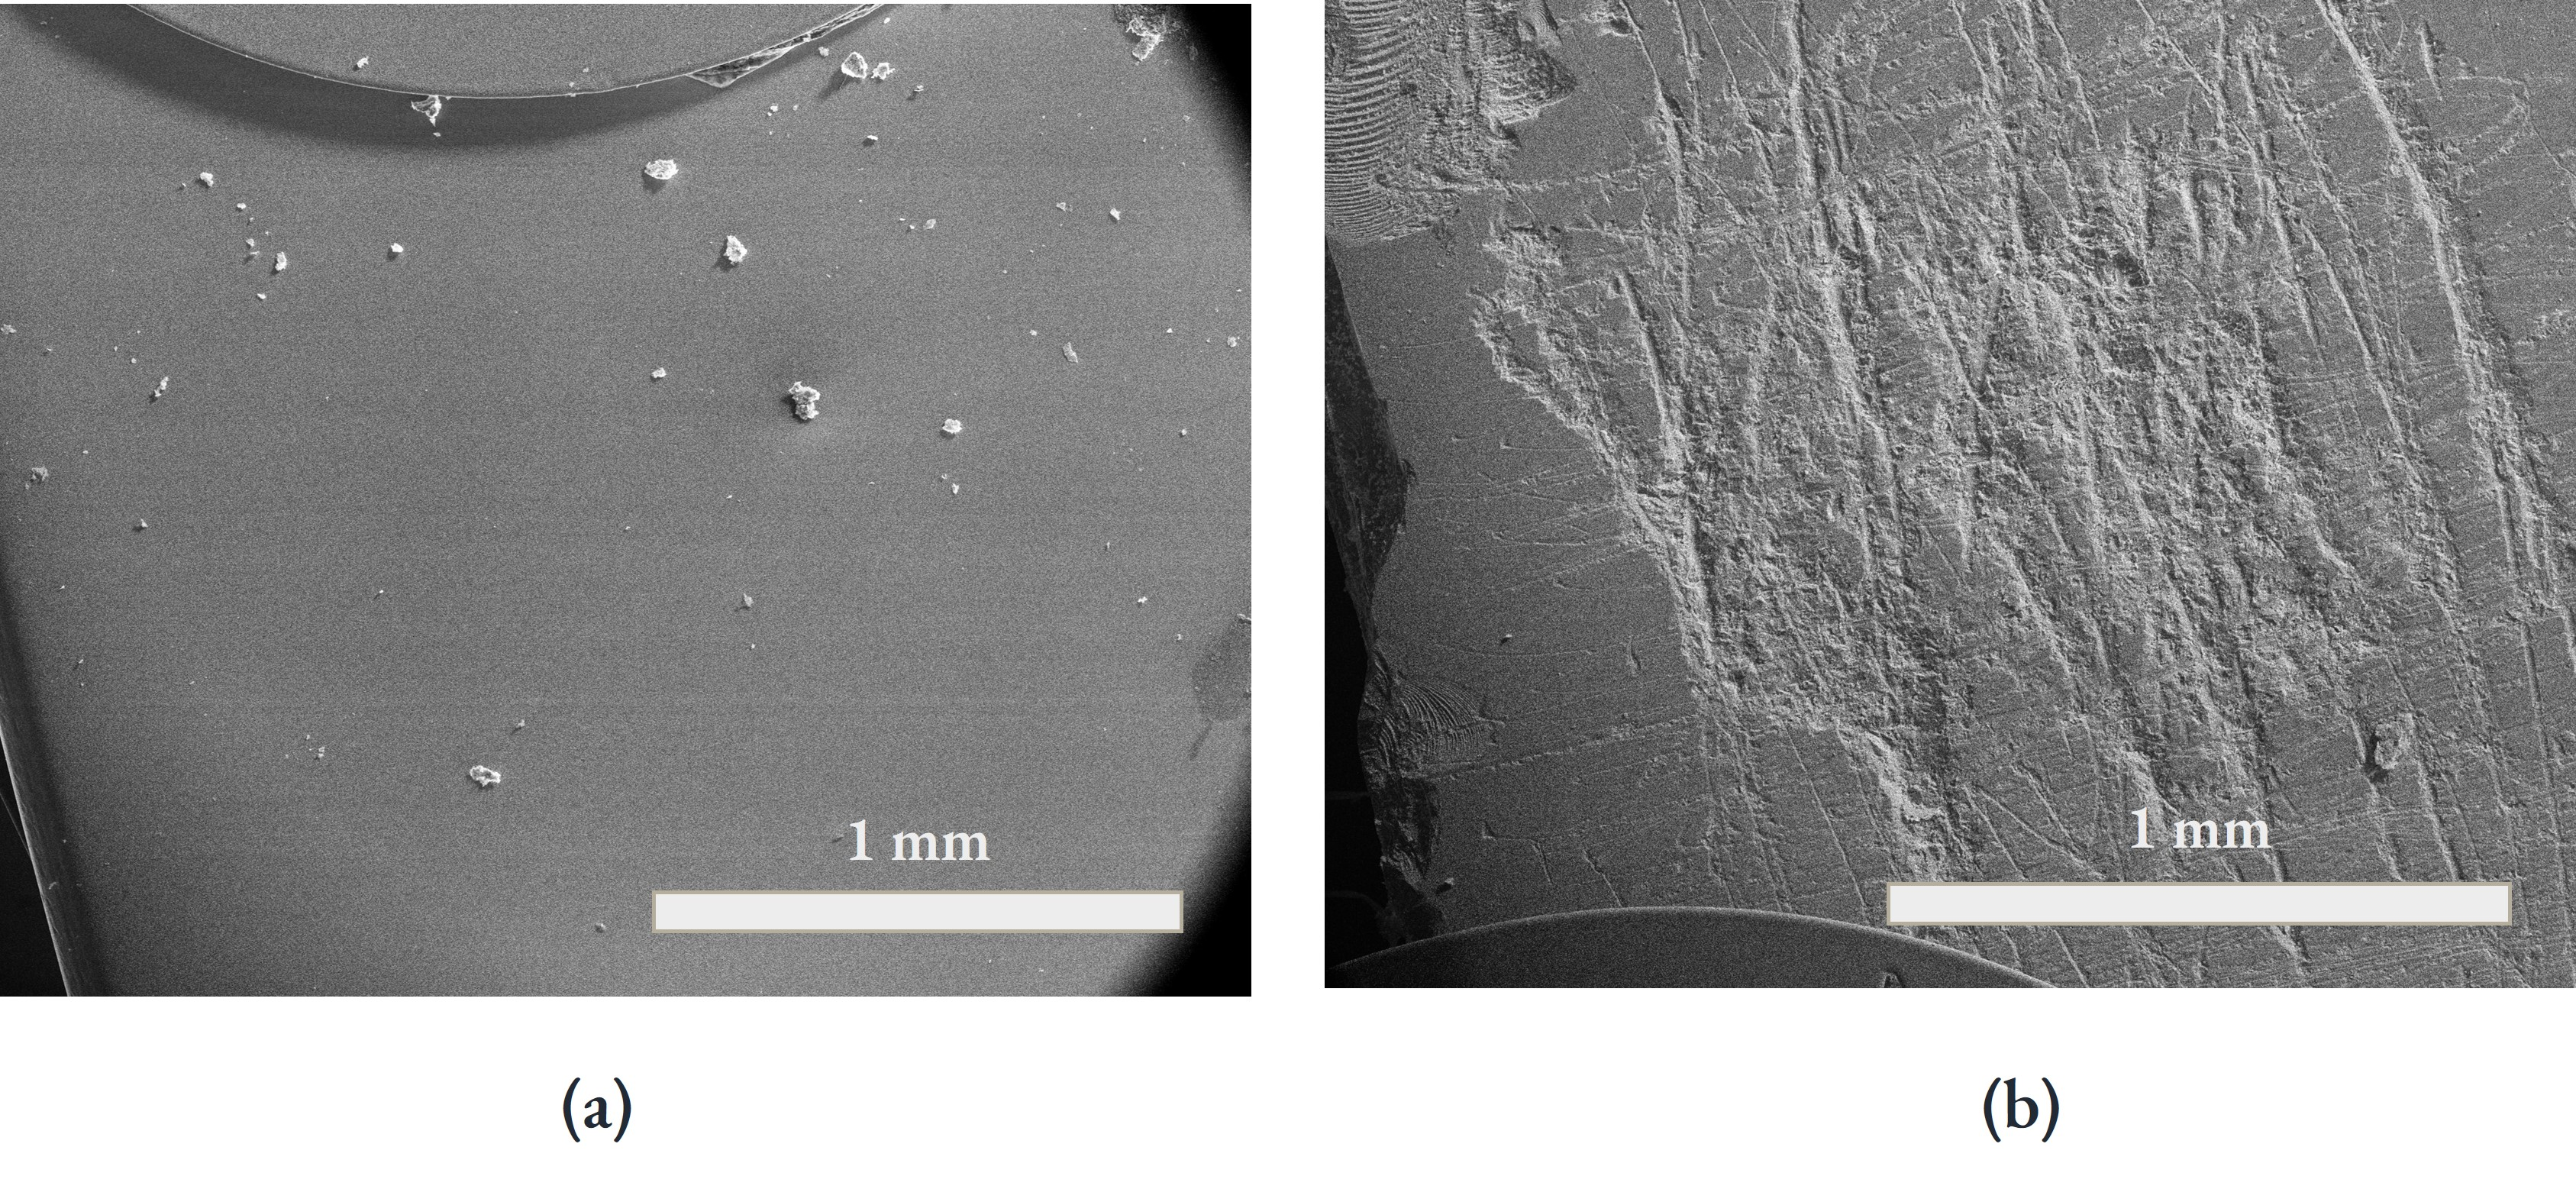
\includegraphics[width=.99\textwidth]{figures/SE_images/Overview_GaAs_GaSb.jpg}
    \caption{
        Overview of the GaAs and GaSb specimen.
        The spectra are acquired in the middle of the images.
        Panel (a) is GaAs, and panel (b) is GaSb.
        The GaSb wafer have areas which are very scratched, but also areas which are smooth.
    }
    \label{fig:SE_images:Overview_GaAs_GaSb}
\end{figure}

\begin{figure}[phtb]
    \centering
    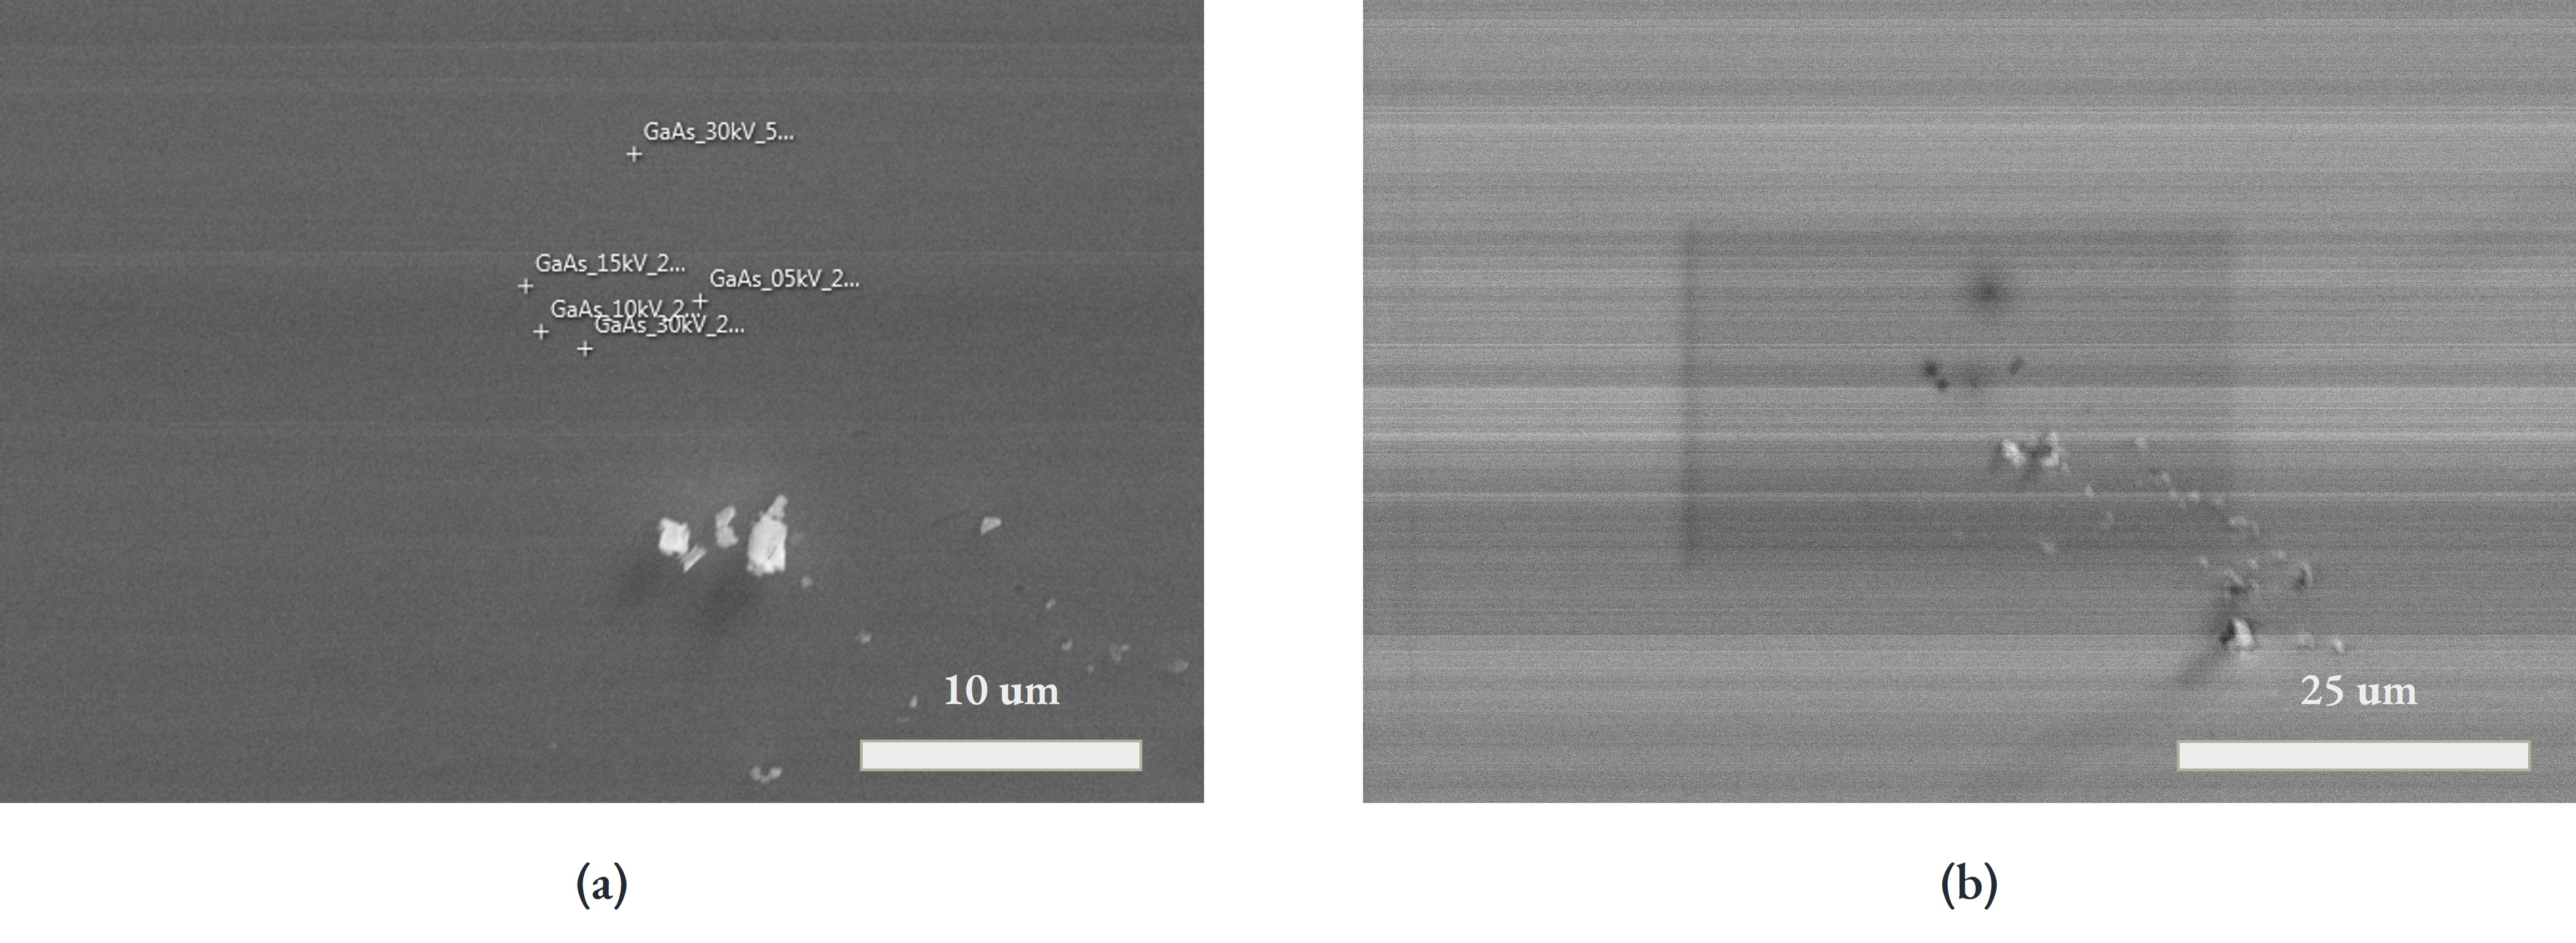
\includegraphics[width=.99\textwidth]{figures/SE_images/GaAs_close.jpg}
    \caption{
        Close up of the GaAs specimen.
        Annotated in panel (a) are the areas which were analyzed.
        Panel (b) is a zoomed out view of the area in panel (a), after the spectra have been acquired.
        This image shows both beam damage from the focused probe beam as black dots, and the whole area from the scanning as a darker square.
    }
    \label{fig:SE_images:GaAs}
\end{figure}


\begin{figure}[htbp]
    \centering
    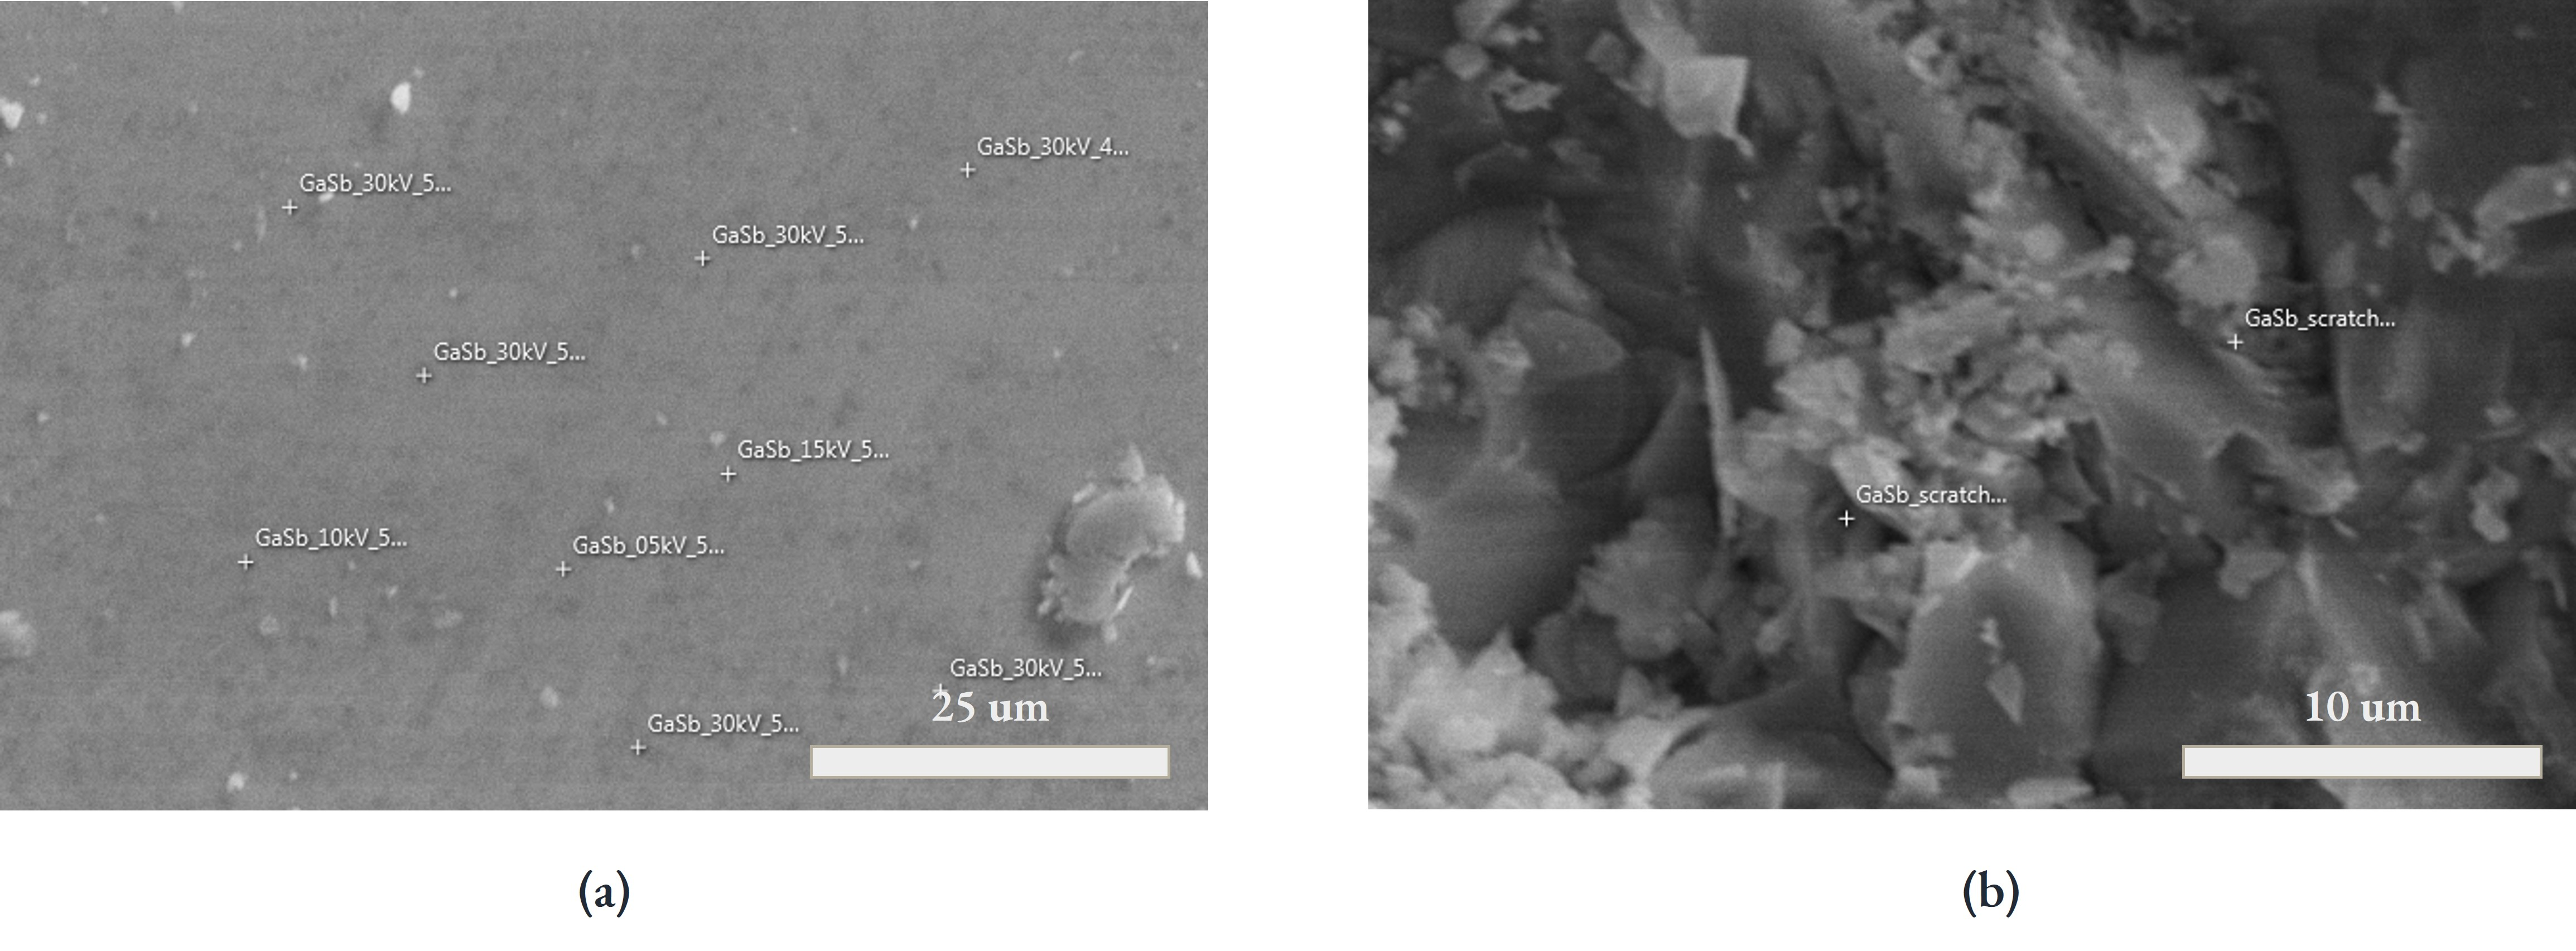
\includegraphics[width=.99\textwidth]{figures/SE_images/GaSb_close.jpg}
    \caption{
        Close up of the GaSb specimen, where the point spectra were acquired.
        Panel (a) is the polished area, and panel (b) is the scratched area.
        Both panels are annotated with the areas which were analyzed.
    }
    \label{fig:SE_images:GaSb}
\end{figure}


% \begin{figure}[htbp]
%     \centering
%     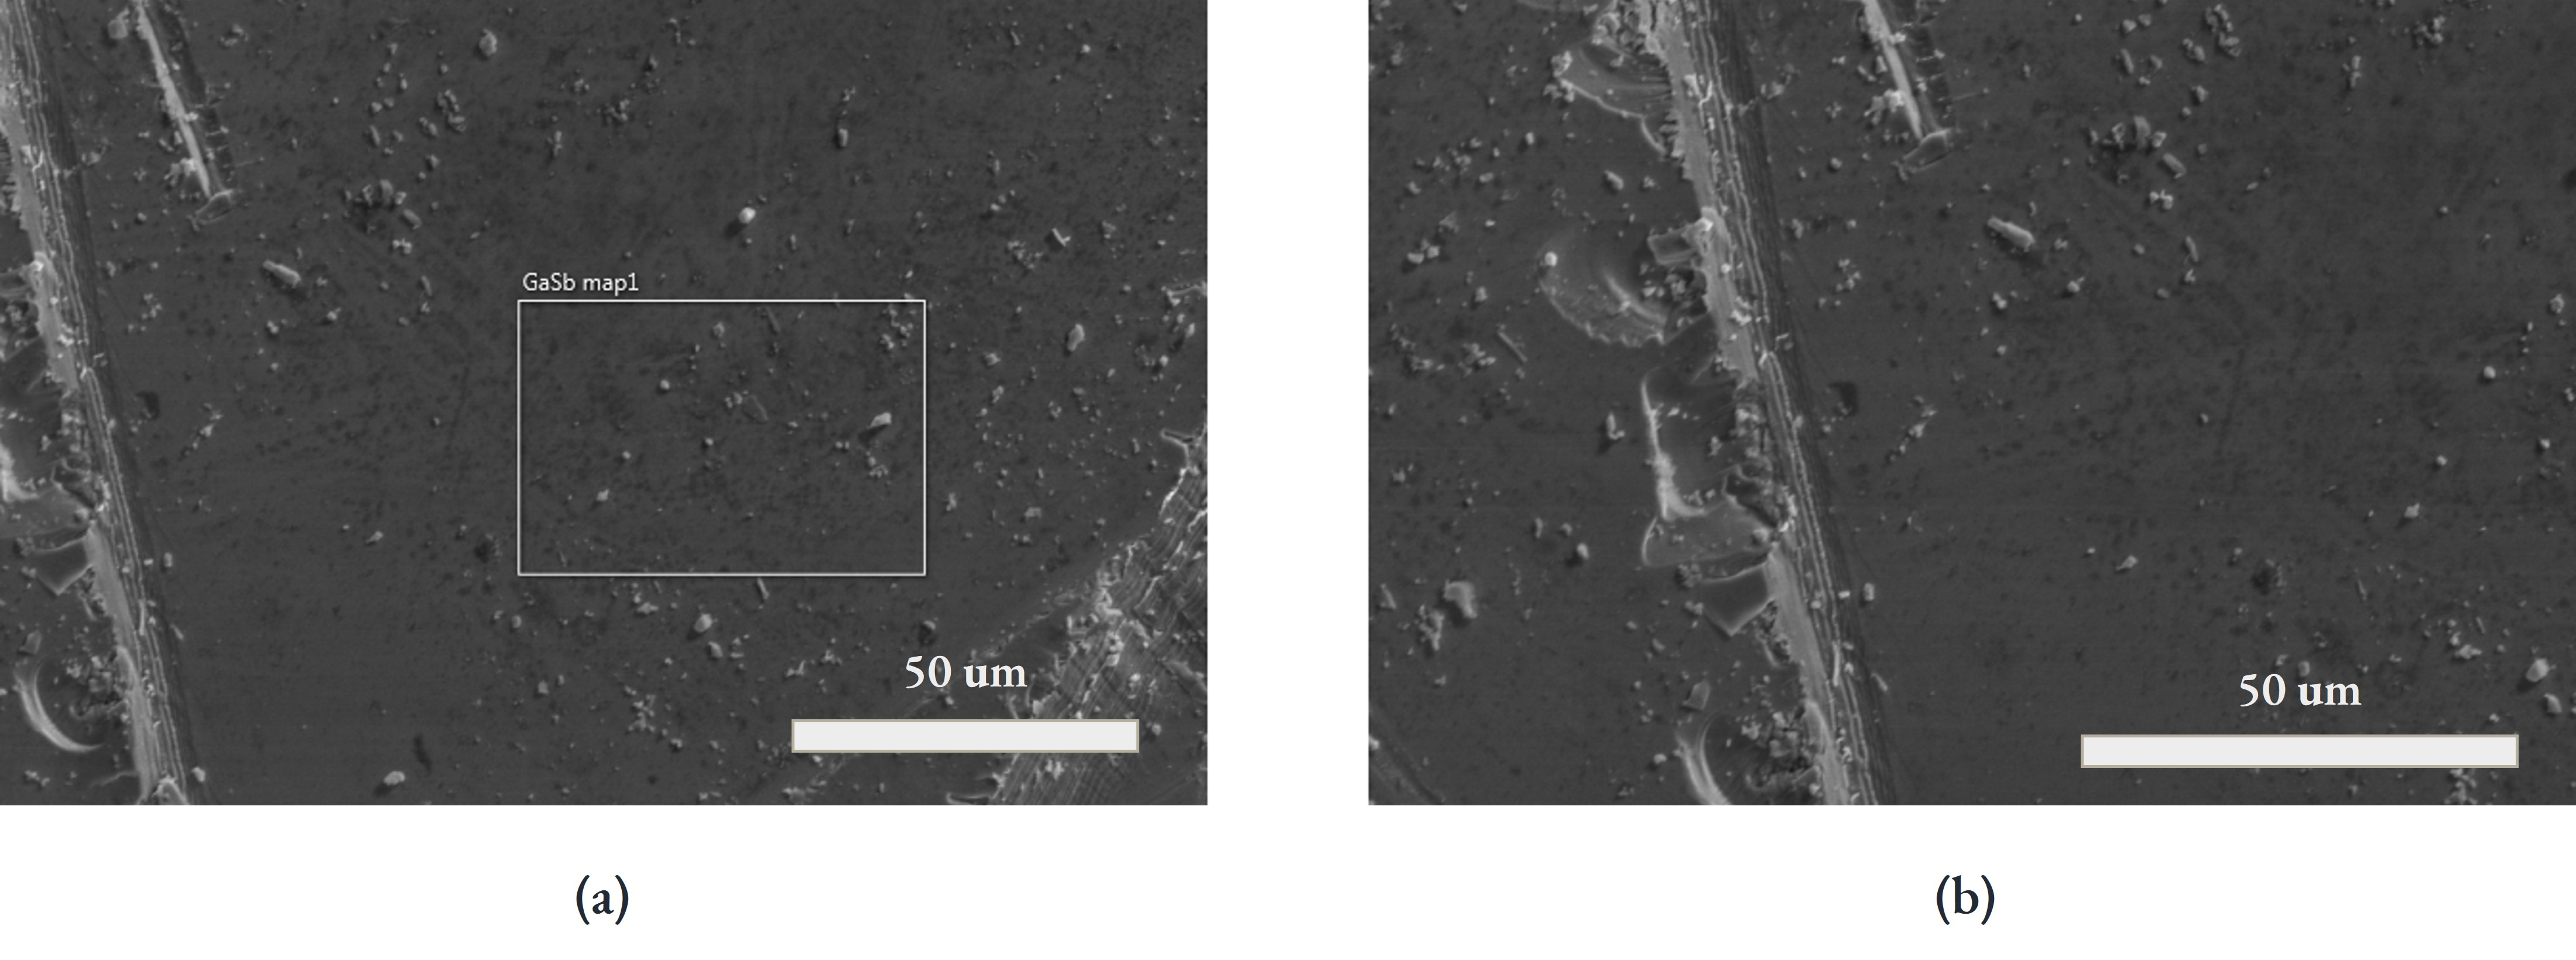
\includegraphics[width=.95\textwidth]{figures/SE_images/GaSb_map.jpg}
%     \caption{
%         Close up of the GaSb specimen, where the map spectra were acquired.
%         Panel (a) is map 1 (within the rectangle), and panel (b) is map 2 (the whole image).
%         Map 2 includes one scratched line in the analyzed area.
%     }
%     \label{fig:SE_images:GaSb_map}
% \end{figure}
















\section{Instruments}
\label{method:instruments}

The acquisition of the spectra was done with an Oxford Instruments Xmax$^N$ $80$ mm$^2$ silicon drift detector for EDS, equipped on a SEM Apreo from FEI.
The Apreo is a field emission SEM, which in addition to the EDS sensor has an Everhart-Thornley detector, in-lens detectors for SE and BSE, a directional BSE detector, and a navigation camera.
In this work, the ET detector was used to verify that the areas studied were clean, flat and representative.
The maximum accelerating voltage is $30$ kV, and the maximum beam current is $400$ nA.
During this work, the acceleration voltage has been in the range $5-30$ kV, and the beam current has been in the range $25-400$ pA.
The acquisition settings used in this study are listed in \cref{tab:method:acquisition_settings:voltage} and \cref{tab:method:acquisition_settings:other}.
The instrument is located at the NTNU NanoLab, a NorFab facility.


The details about the EDS detector is from \cite{xmaxn_datasheet} and the description provided by NanoLab.
The Oxford Xmax$^N$ SDD has an $80$ mm$^2$ active area. %, which gives a solid angle of $0.03409$ sr at WD=$10$ mm.
The specifications list the following FWHM energy resolutions at $50$k cps: Mn K$\alpha$ at 127 eV, F  K$\alpha$ at 64 eV, and C  K$\alpha$ at 56 eV.
Giving the specifications like this is in compliance with the ISO 15632:2012 standard \cite{iso_qc_15632}.
% The detector is from before 2010, with a claimed count rate of $> 500$k cps and throughout $> 200$k cps \cite{xmaxn_datasheet}.
All elements from Be to Cf can be analyzed, as the detector has a thin polymer window.
The detector is mounted at $35$\textdegree.
The process time settings range from $1$ to $6$, and they have no further explanation of what the number indicates.
The detector is operated with the AZtec software, provided by Oxford Instruments NanoAnalysis \cite{aztec_manual}.



\section{Acquisition settings in the measurement series}
\label{method:acquisition_settings}

The settings selected are based on Goldstein \cite{goldstein_scanning_2018} and the goal of analyzing spectra with varying acquisition parameters.
The acquisition is divided into four groups, where the two first are acquisition with varying acceleration voltage and constant beam current.
(A) is the voltage series on GaAs, and (B) is the voltage series on GaSb.
The two other series test parameter variation on the GaSb specimen: (C) is with varying PT, (D) is with varying $i_b$, PT, and $E_0$.
The voltage series is used to study the effect of the acceleration voltage, to figure out if an optimal voltage exists.
The other acquisition settings tested variations of different settings on the GaSb specimen, to see if any of these settings could improve the quality of the spectra.
An overview of all acquisition settings for each spectrum is given in \cref{tab:method:acquisition_settings:all_spectra}.
The acquisition settings are listed in \cref{tab:method:acquisition_settings:voltage} and \cref{tab:method:acquisition_settings:other}.
Dead time (DT) and input count rate (ICR) is a function of the other settings.


% constant variables
Some variables were kept constant during all the acquisition.
The tilt of the specimen was kept at $0$\textdegree, and thus the TOA was $35$\textdegree, because of the mounted angle of the detector.
The live time for each spectrum was $120$ s, except for two of the spectra in the (D) series, which had a high DT.
The range of the spectra was $0-20$ keV, with a scale of $10$ eV/channel.

\begin{table}[phtb]
    \begin{center}
        \caption{
            Experimental settings of acquired and used spectra in this work.
            % \brynjar{Comment from Ton: Add a column with spectra names, e.g. A, B, C, D.}
            The spectra are divided into five groups: (A) voltage series GaAs, (B) voltage series GaSb, (C) different PT, (D) different $i_b$, $E_0$, and PT, and (E) maps.
            Parameters not specified are as in \cref{tab:method:acquisition_settings:voltage}.
        }
        \renewcommand*{\arraystretch}{1.2}
        \label{tab:method:acquisition_settings:all_spectra}
        \begin{tabular}{lllllllp{3.5cm}}
            \hline
            \textbf{Group}                     & \textbf{Sample} & \textbf{$E_0$} & \textbf{$i_b$} & \textbf{PT} & \textbf{ICR} & \textbf{DT} & \textbf{Comment}    \\
                                               &                 & [kV]           & [pA]           &             & [k counts]   & [\%]        &                     \\
            \hline
            \emph{GaAs $E_0$ series}           &                 &                &                &             &              &             &                     \\
            A                                  & GaAs            & 5              & 25             & 6           & 0.88         & 3           &                     \\
            A                                  & GaAs            & 10             & 25             & 6           & 1.75         & 6           &                     \\
            A                                  & GaAs            & 15             & 25             & 6           & 3.3          & 12          &                     \\
            A                                  & GaAs            & 30             & 25             & 6           & 8            & 25          &                     \\
            A                                  & GaAs            & 30             & 50             & 6           & 16.4         & 44          & Additional spectrum \\
            \hline
            \emph{GaSb $E_0$ series  }         &                 &                &                &             &              &             &                     \\
            B                                  & GaSb            & 5              & 50             & 6           & 1.08         & 4           &                     \\
            B                                  & GaSb            & 10             & 50             & 6           & 2.3          & 9           &                     \\
            B                                  & GaSb            & 15             & 50             & 6           & 5.7          & 18          &                     \\
            B                                  & GaSb            & 30             & 50             & 6           & 17           & 44          &                     \\
            \hline
            \emph{PT change}                   &                 &                &                &             &              &             &                     \\
            C                                  & GaSb            & 30             & 50             & 4           & 17           & 13          &                     \\
            C                                  & GaSb            & 30             & 50             & 2           & 17           & 7           &                     \\
            C                                  & GaSb            & 30             & 50             & 1           & 17           & 4           &                     \\
            \hline
            \emph{$i_b$, $E_0$, and PT change} &                 &                &                &             &              &             &                     \\
            D                                  & GaSb            & 30             & 400            & 1           & 160          & 28          & Very high counts    \\
            D                                  & GaSb            & 15             & 200            & 6           & 22           & 53          & 61 s live time      \\
            D                                  & GaSb            & 15             & 400            & 6           & 42           & 77          & 59 s live time      \\
            %             & GaSb            & 15             & 400             & 3           & 50           & 25          & Scratched area      \\
            %             & GaSb            & 30             & 25              & 6           & 6.5          & 20          & Scratched area      \\
            % \hline
            % \emph{Maps}                &                 &                &                &             &              &             &                     \\
            % E                          & GaSb            & 15             & 400            & 3           & 43           & 22          & Map 1               \\
            % E                          & GaSb            & 15             & 400            & 3           & 43           & 22          & Map 2               \\
            \hline
        \end{tabular}
    \end{center}
\end{table}


\begin{table}[phtb]
    \begin{center}
        \caption{
            Measurement series A and B, which tested different $E_0$ on GaAs and GaSb.
            All spectra were recorded with 0-20 keV energy range and 2048 channels at working distance 10 mm (optimal for the detector), and the at TOA 35\textdegree.
            %
        }
        \renewcommand*{\arraystretch}{1.2}
        \label{tab:method:acquisition_settings:voltage}
        \begin{tabular}{p{2cm}p{3cm}p{8.6cm}}
            \hline
            \textbf{Setting}    & \textbf{Values}      & \textbf{Comment}                                                                                                                                                                                                                                               \\
            \hline
            Beam energy         & 30, 15, 10, and 5 kV & To study the effect of different $E_0$.                                                                                                                                                                                                                        \\
            % Beam current        & 25 pA (GaAs), 50 pA (GaSb) & Set to get sufficient amount of counts and maximum DT around 30\% at 30 kV. Then kept constant when $E_0$ was decreased in the voltage series. Different beam current for the specimen was chosen to see the effects on Ga. \\
            Beam current        & 25 pA or 50 pA       & 25 pA for GaAs and 50 pA for GaSb. Set to get sufficient amount of counts and maximum DT around 30\% at 30 kV. Then kept constant when $E_0$ was decreased in the voltage series. Different beam current for the specimen was chosen to see the effects on Ga. \\
            Process time        & 6 (maximum)          & Set to the highest to influence the acquisition as little as possible, i.e. giving the highest energy resolution.                                                                                                                                              \\
            DT GaAs             & 25\%, 12\%, 6\%, 3\% & DT is not a setting, but a result of other settings. The low DT at the lower $E_0$ was due to fewer counts.                                                                                                                                                    \\
            DT GaSb             & 44\%, 18\%, 9\%, 4\% &                                                                                                                                                                                                                                                                \\
            Data type           & PointID              & The voltage series was only done with PointID, while mapping was tested in the measurement series summarized in \cref{tab:method:acquisition_settings:other}.                                                                                                  \\
            Live time           & 120 s                & To get sufficient amount of counts.                                                                                                                                                                                                                            \\
            Additional spectrum & GaAs, 30 kV, 50 pA   & An additional spectra on GaAs with the same settings at the 30 kV spectrum of GaSb. Taken to directly compare the 30 kV spectra.                                                                                                                               \\

            \hline
        \end{tabular}
    \end{center}
\end{table}
%%%%%%%%%%%%%%%%%%%%%%%%%%%%%%%%%%%%%%%%%%%%%%%%%%%%%%%%%%%%%%%%%%%%%%%%%%%%%%%%%%%%%%%%
%%%%%%%%%%%%%%%%%%%%%%%%%%%%%%%%%%%%%%%%%%%%%%%%%%%%%%%%%%%%%%%%%%%%%%%%%%%%%%%%%%%%%%%%
%%%%%%%%%%%%%%%%%%%%%%%%%%%%%%%%%%%%%%%%%%%%%%%%%%%%%%%%%%%%%%%%%%%%%%%%%%%%%%%%%%%%%%%%
\begin{table}[phtb]
    \begin{center}
        \caption{
            Measurement series B and C, which tested variation in $i_b$, PT, and $E_0$.
            These measurements were only done on the GaSb specimen.
            Data type, live time, energy range, channels, WD, and TOA as in \cref{tab:method:acquisition_settings:voltage}.
        }
        \renewcommand*{\arraystretch}{1.2}
        \label{tab:method:acquisition_settings:other}
        \begin{tabular}{p{2cm}p{3cm}p{8.6cm}}
            \hline
            \textbf{Setting} & \textbf{Values}     & \textbf{Comment}                                                                               \\
            \hline
            Beam energy      & 15 and 30 kV        & Further inspect the effect of the Sb K-peaks just below 30 kV.                                 \\
            Beam current     & 50, 200, and 400 pA & To study ICR and DTs, with values given in \cref{tab:method:acquisition_settings:all_spectra}. \\
            Process time     & 1, 2, 4, and 6      & To study the effect of PT, e.g. on energy resolution and coincidence events.                   \\
            % Data type        & PointID and Map     & Compare results from a point and a map, with eventual denoising in the map.                    \\
            %  &                     &                                                                                                       \\
            %  &                     &                                                                                                       \\
            %  &                     &                                                                                                       \\
            \hline
        \end{tabular}
    \end{center}
\end{table}





















\clearpage

\section{Data treatment}
\label{method:data_treatment}

The data treatment is divided into three parts: acquisition and extraction, performance parameters, and quantification.
All the notebooks run on Python 3.10, with the packages listed in \cref{tab:method:packages}.
All dependencies were installed using the package manager Mamba 1.4.0, with Conda 22.11.1.
When contributing to HyperSpy, the developer version of HyperSpy was installed using pip 23.0.
One notebook is attached in the appendix of this thesis, and both this and the other notebooks are available at GitHub in the repositories \href{https://github.com/brynjarmorka/sem-eds-qc}{"sem-eds-qc"}\footnote{"qc" = quality control} and \href{https://github.com/brynjarmorka/eds-sem-bulk-corrections}{"eds-sem-bulk-corrections"}. 

\begin{table}[hbtp]
    \begin{center}
        \caption{
            The Python packages.
            All dependencies was installed using the package manager Mamba 1.4.0, with Conda 22.11.1.
            When contributing to HyperSpy, the developer version of HyperSpy was installed using pip 23.0.
        }
        \renewcommand*{\arraystretch}{1.2}
        \label{tab:method:packages}
        \begin{tabular}{p{4cm}p{10.6cm}}
            \hline
            \textbf{Package name} & \textbf{Description}                                          \\
            \hline
            HyperSpy 1.7.4        & Multi-dimensional data analysis toolbox.                      \\
            Plotly 5.13.1         & Interactive, open-source, and browser-based graphing library. \\
            Numpy 1.23.5          & Scientific computing with Python.                             \\
            Pandas 1.5.3          & Data analysis package.                                        \\
            JupyterLab 3.6.2      & Web-based interactive development environment.                \\
            SciPy 1.10.1          & Scientific computing with Python.                             \\
            Matplotlib 3.7.1      & Static, animated, and interactive visualizations.             \\
            \hline
        \end{tabular}
    \end{center}
\end{table}


\subsection{Acquisition and extraction - AZtec}
\label{method:data_treatment:aztec}

Acquisition and extraction is done with AZtec version 5.0, provided by Oxford Instruments NanoAnalysis \cite{aztec_manual}.
Steps for acquisition is described in Appendix A of Lundeby \cite{lundeby_improving_2019}.
The "SEM EDS" setting was selected.
Point measurements was done with "Point \& ID".
%, and map measurements was done with "Map".
The point spectra was extracted as ".emsa" files.
% The data from the map spectra was exported as ".emsa", ".raw", ".rpl", and ".txt" files, which was merged to one ".hdf5" file with the script from Lundeby \cite[A.3]{lundeby_improving_2019}.
% The merge script and the relevant Appendix from Lundeby is available at the author of this thesis' GitHub \verb|\cref{} or link|.

Summarized, the acquisition and extraction in AZtec was done as follows:
\begin{enumerate}
    \item "SEM EDS" setting selected.
    \item Data type selected as "Point \& ID".
    \item Navigated to the area of interest with the ET detector.
    \item Selected settings for the acquisition, see \cref{tab:method:acquisition_settings:all_spectra}.
    \item Started the acquisition.
    \item Verified the element with the spectrum and an interactive periodic table.
    \item AZtec calculated the composition.
    \item The spectra were extracted for notebook analysis.
\end{enumerate}


Initial qualitative analysis was done with the AZtec software, to get an overview of the spectra.
All spectra were quantitatively analyzed with the AZtec software to later compare with HyperSpy and the notebooks developed in this thesis.
The "SEM EDS" quantification in AZtec give the composition and the calculated k-ratios for each element.
Additionally, quantification with the "TEM EDS" setting in AZtec was tested, where both the composition and calculated k-factors were extracted.
This "TEM EDS" step was done to verify that AZtec does use matrix corrections, and to get the k-factors for CL quantification with HyperSpy.






\subsection{Performance parameters - Jupyter notebooks}
\label{method:data_treatment:notebook}

A Jupyter notebooks was developed for the calculation of SEM EDS performance parameters, i.e. the top and middle row of \cref{fig:intro:parameters}.
The notebooks for performance parameters calibrates the spectrum, and calculates: the Duane-Hunt limit, the energy resolution, the Fiori P/B, peak intensities, FWHMs, peak deviations, and specified peak ratios.
The list below describes the steps in the notebooks, which are included as headers in the notebooks.
See \hyperref[appendix:performance]{Appendix A} for the notebook, or \href{https://github.com/brynjarmorka/sem-eds-qc/blob/main/SEM_EDS_performance_parameters.ipynb}{view it on GitHub}.
The performance parameter notebook does the following steps:

\begin{enumerate}
    \item Import the packages
    \item Select spectra, and specify settings like $i_b$, $E_0$, ICR, and PT
    \item Import the data with HyperSpy, set the elements in the spectrum, and slice off the noise peak
    \item Calculate the Duane-Hunt limit, and slice the spectrum to the limit
    \item Make a model of the spectrum, and fit it to the data
    \item Calibrate the offset and scale
    \item Calibrate the energy resolution
    \item Calibrate the energy and width of the peaks
    \item Calculate Fiori P/B, peak intensities, FWHMs, and peak deviations
    \item Calculate the relevant peak ratios
    \item Save the results in a DataFrame in a ".csv" file
\end{enumerate}










\subsection{Quantification - HyperSpy and Jupyter notebooks}
\label{method:data_treatment:quantification}

The different quantification routines and bulk corrections performed in the notebooks are made available at the author of this thesis' GitHub in the repository \href{https://github.com/brynjarmorka/eds-sem-bulk-corrections}{"eds-sem-bulk-corrections"}, under the user "brynjarmorka"\footnote{\url{https://github.com/brynjarmorka/eds-sem-bulk-corrections/}}.
The initial quantification was done with the intensity ratio method, where the intensities were extracted from a model fit of the spectrum through HyperSpy.
The next paragraphs describe: the Cliff-Lorimer (CL) method in HyperSpy, the calculation of the ZAF absorption correction, and the implementation of the XPP model.

% CL
The CL quantification in HyperSpy was done according to the documentation.
The Jupyter notebook with the quantification is named \href{https://github.com/brynjarmorka/eds-sem-bulk-corrections/blob/main/quant-of-SEM-EDS-with-Cliff-Lorimer.ipynb}{quant-of-SEM-EDS-with-Cliff-Lorimer.ipynb}.
The spectrum was loaded, and the elements were set.
The data was sliced after the noise peak at $0.2$ eV, and at the $E_0$ from the metadata.
A model, with a polynomial background and Gaussian peaks, were made and fitted.
The intensities of the peaks were extracted, and given as input to the CL quantification routine.
The k-factors, calculated by AZtec based on the element and $E_0$, were also given as input to the Cliff Lorimer routine, and are tabulated in \cref{tab:results:TEM_quantification}.
The different absorption correction thicknesses were tested for a range of thicknesses between $50$ nm and $10$k nm.
The results, as compositions, were plotted for inspection, and saved in an external file.

% ZAF
The ZAF absorption corrections (A) use the intensities from a model fit, and applies absorption corrections to these.
A Jupyter notebook with the ZAF absorption correction is named \href{https://github.com/brynjarmorka/eds-sem-bulk-corrections/blob/main/ZAF-absorption-correction-model.ipynb}{ZAF-absorption-correction-model.ipynb}.
To calculate A, the code needs some factors. 
The average density was calculated with \verb|density_of_mixture()| from HyperSpy.
The electron range is calculated with an implementation of the Kanaya-Okayama parameterization.
The average depth is calculated as the maximum electron range, divided by 2, 3, or 4.
The path length is calculated with the TOA and the average depth.
With these factors, the measured intensity is corrected with \cref{eq:theory:quantitative:absorption}, to get an approximation for the generated intensity. 
The generated intensities are used to calculate corrected compositions, which are given in atomic percent.
In the end, the results are saved in an Excel file.


% XPP
The XPP model is implemented in Python files, which are imported into Jupyter notebooks.
The implementation of the equations are separated into smaller functions in the Python files, so that they are more flexible and easier to reuse.
The Python files contains many functions which does small steps, and thus the code is easier to reuse and debug.
Unlike the performance parameters, the XPP model is exemplified through two notebooks.
One notebook in the repository is used to apply the model on the acquired spectra, and another notebook is used to plot different parts of the model.
The Python files 
\href{https://github.com/brynjarmorka/eds-sem-bulk-corrections/blob/main/PAP_functions/PAP_parameterization.py}{PAP-parameterization.py}, 
\href{https://github.com/brynjarmorka/eds-sem-bulk-corrections/blob/main/PAP_functions/PAP_helper_functions.py}{PAP-helper-functions.py}, and 
\href{https://github.com/brynjarmorka/eds-sem-bulk-corrections/blob/main/PAP_functions/PAP_area_F.py}{PAP-area.py} are for the calculation of the XPP model.
The 
\href{https://github.com/brynjarmorka/eds-sem-bulk-corrections/blob/main/PAP_functions/PAP_parameterization.py}{PAP-parameterization.py}
file calculates $F(\chi)$ and $f(\chi)$, see \cref{sec:theory:quantitative:pap:emergent_intensity} and \cref{eq:theory:quantitative:pap:general_principle:f_absorption_correction}.
The 
\href{https://github.com/brynjarmorka/eds-sem-bulk-corrections/blob/main/PAP_functions/PAP_helper_functions.py}{PAP-helper-functions.py}
file contains helper functions, e.g. for getting the theoretical energy of a line, and converting at.\% to wt.\%.
The 
\href{https://github.com/brynjarmorka/eds-sem-bulk-corrections/blob/main/PAP_functions/PAP_area_F.py}{PAP-area.py}
file calculates $F$, see \cref{theory:quantitative:pap:calculation_of_F}.
The code is based on the PAP paper \cite{pap_1991}, and all the equations are described in \cref{theory:quantitative:pap}.
Additionally, all the equations are written out with \LaTeX in the notebooks, and every function has a NumPy-style docstring.
The files and notebooks contains many lines and are cannot be printed practically, and thus the code is not attached, but it is available under a MIT license at the author of this thesis' GitHub, in the repository \href{https://github.com/brynjarmorka/eds-sem-bulk-corrections}{"eds-sem-bulk-corrections"}.

% The XPP files
